
\begin{figure}
	\centering
	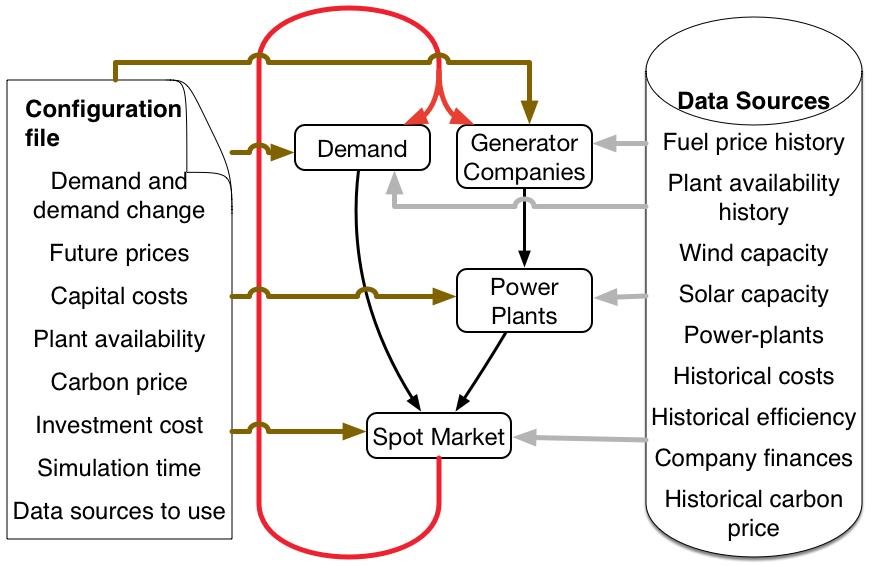
\includegraphics[width=0.97\linewidth]{figures/System_overview_large}
	\caption{System overview of agent-based market model.}
	\label{fig:systemoverview}
\vskip -6mm
\end{figure}


\begin{figure*}[h]
	\centering
	\begin{subfigure}[b]{0.33\textwidth}
		\centering
		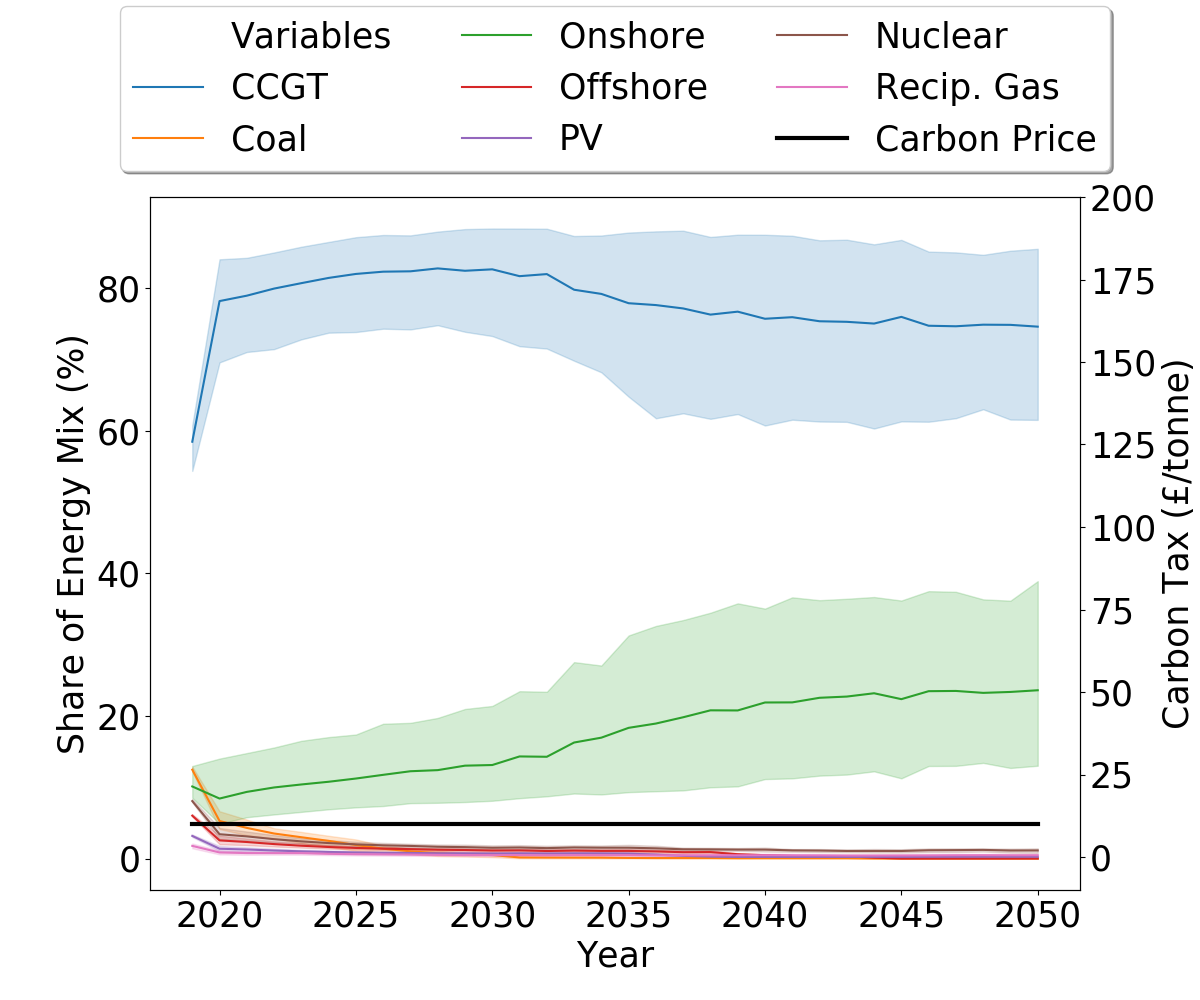
\includegraphics[width=\textwidth]{figures/scenarios/demand099-carbon10-datetime.png}
		\caption[Network2]%
		{\small \textsterling10 carbon tax.}
		\label{fig:demand99carbon10}
	\end{subfigure}
	\hfill
	\begin{subfigure}[b]{0.33\textwidth}  
		\centering 
		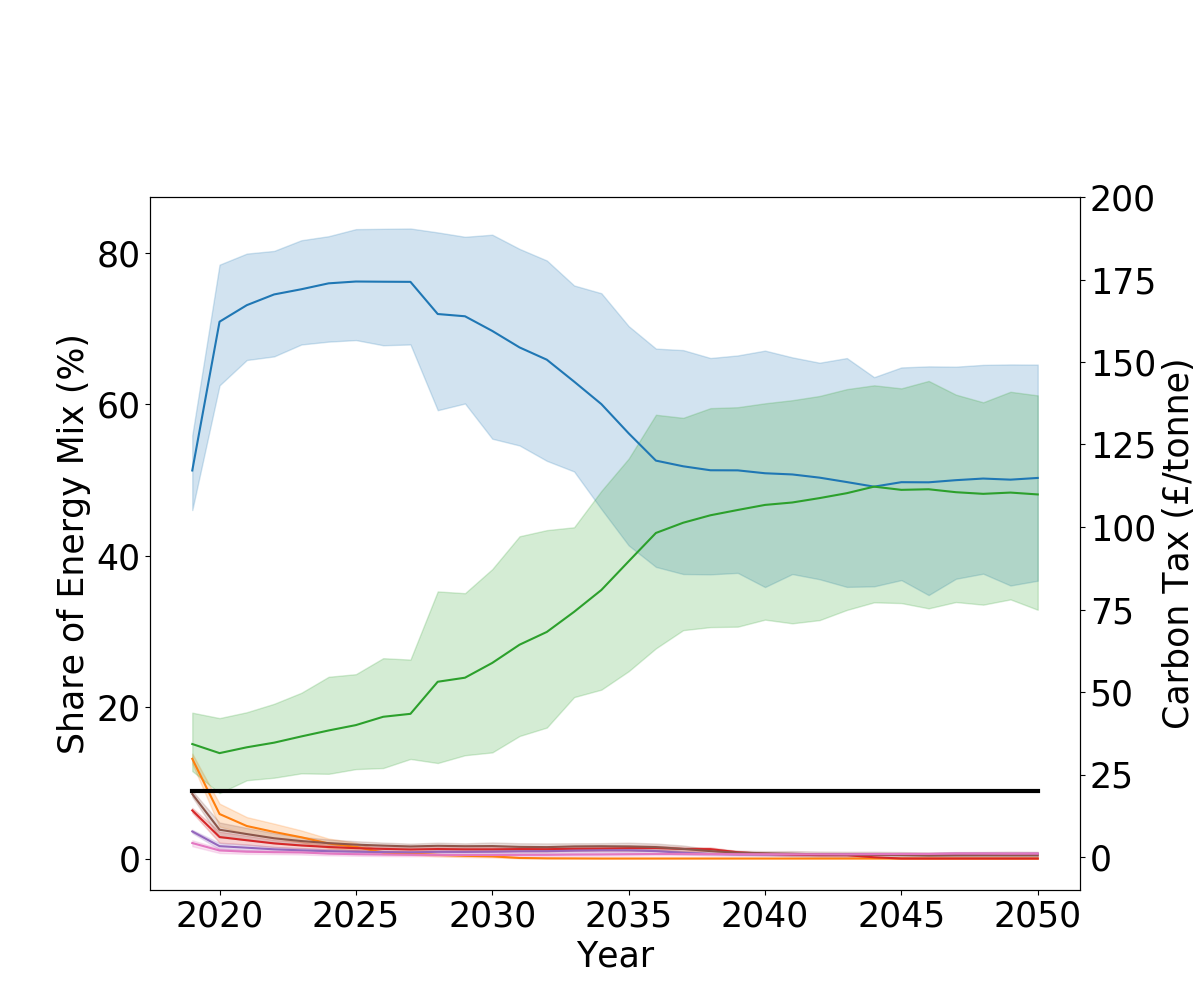
\includegraphics[width=\textwidth]{figures/scenarios/demand099-carbon20-datetime.png}
		\caption[]%
		{\textsterling20 carbon tax.}
		\label{fig:demand99carbon20}
	\end{subfigure}
	\begin{subfigure}[b]{0.33\textwidth}
		\centering
		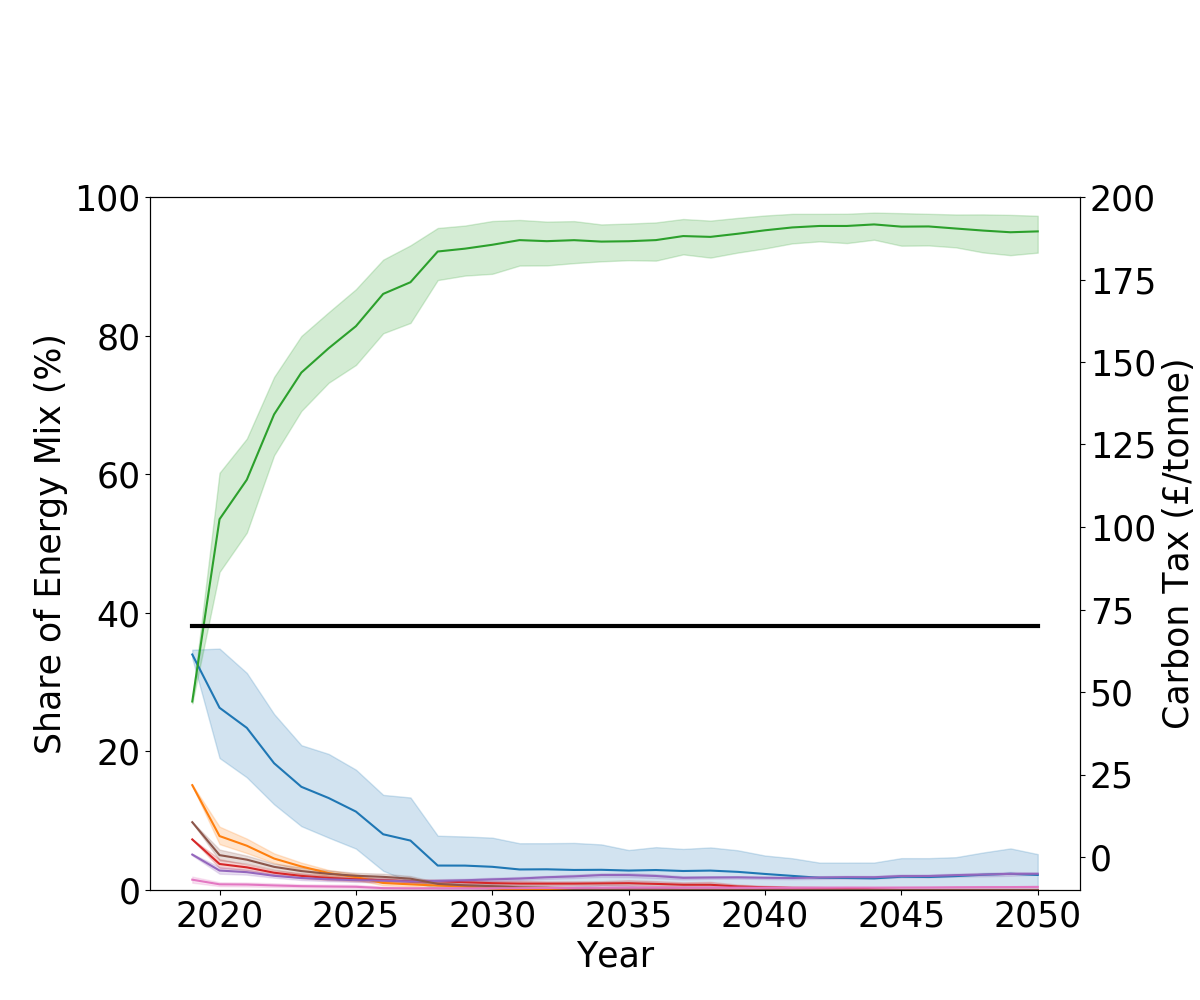
\includegraphics[width=\textwidth]{figures/scenarios/demand099-carbon70-datetime.png}
		\caption[Network2]%
		{\small \textsterling70 carbon tax.}
		\label{fig:demand99carbon70}
	\end{subfigure}
	\caption{Scenarios from 2020 to 2050 with varying carbon tax.}
\end{figure*}


The agent-based model is made up of five significant parts: the agents which are made up of the generation companies (GenCos) and demand agents; power plants and a market operator which controls the spot market. How these parts interact are displayed in Figure \ref{fig:systemoverview}. The relevant data sources are also provided here.

We initialise the United Kingdom with our model with exemplar data from the UK. We model every single power plant in operation in the year 2018, which are owned by their respective generation companies. Individual historical power plant costs are estimated from levelized cost of electricity (LCOE) \cite{Dale2013, IEA2015,IRENA2018}, whereas future and present power plant costs are taken from the department of business and industrial strategy \cite{Department2016}. The variable operation and maintenance cost was defined stochastically to model the changing costs per project. A uniform distribution was chosen to provide sufficient variance between projects.

The demand agent is modelled as a single aggregated demand, split up into 20 segments of a load duration curve (LDC), enabling us to increase speed of computation whilst maintaining accuracy. An LDC is defined as a yearly load sorted in order of magnitude. 

We model the influence of outages using availability data for gas, coal, photovoltaic, offshore and onshore power generators \cite{Ltd2016, Hunt2015, carroll-j}. Historical availabilities are modelled for older gas, coal and hydro power plants \cite{AlbertaSystemElectricOperator2016}. Capacity factors were taken as an average of the UK for solar and wind \cite{Pfenninger2016, Staffell2016}. Where capacity factors is defined as the ratio of electrical output over a given time period over the maximum possible electrical energy output. 

The generation companies make electricity bids each year for each of their power plants. The market operator then matches demand with supply in order of price, also known as merit-order dispatch. We model a uniform pricing market, where each of the companies are paid the highest accepted bid.

GenCos have the ability to invest every year in new power plants based on the expected net present value (NPV) of each type of power plant. NPV is a summation of the present value of a series of present and future cash flow. The NPV calculation is dependent on a stochastic representation of GenCos predictions of fuel, carbon and electricity price and demand.

Each GenCo has a separate weighted average cost of capital (WACC), which is the rate that a company is expected to pay on average for its stock and debt, this is used as the discount rate in the NPV calculation \cite{KincheloeStephenC1990TWAC}. The WACC is modelled as a stochastic variable, with a Gaussian distribution and a $\pm3\%$ standard deviation, with values of 5.9\% for non-nuclear power plants, and 10\% for nuclear power plants \cite{KPMG2017, Paper2012}. 

The model took yearly time-steps to limit the impact on computation time, however, to model the intermittency of renewable generation, we correlated demand with the respective capacity factor, enabling for example, solar and wind to only contribute a certain capacity to their load curve.

Stochasticity of fuel price within a year was also modelled, to take into account difference in hedging strategies and chance. An ARIMA model \cite{ARIMA} was fit to historic coal and natural gas prices.



